\documentclass[]{beamer}
\usetheme{Dresden}

\usepackage{graphicx}
\usepackage{listings}
\usepackage{menukeys}
%\usepackage{hyperref} % for URLs, already included in beamer
\usepackage{lmodern} %% allow bold keywords
\usepackage{color}

\definecolor{darkgreen}{rgb}{0,0.5,0}

\lstset{language=Java,
	basicstyle=\ttfamily\footnotesize,
	keywordstyle=\color{purple},
	commentstyle=\color{darkgreen},
	numberstyle=\tiny\color{gray},
	stringstyle=\color{blue},
	tabsize=4,
	showstringspaces=false,
	breaklines=true,
	keepspaces=true,
	numbers=left,
	escapechar=@
}

\usepackage[ngerman]{babel}

\begin{document}
\title{Zwischenpr\"asentation Geek-Shop}
\author{Softwaretechnologie-Projekt 2014 Gruppe 30}
\date{27. November 2014}

\begin{frame}
\titlepage
\end{frame}

\begin{frame}
\frametitle{Gruppenmitglieder}
\begin{tabular}{rp{10cm}}
Chefprogrammierer: & Sebastian D\"oring \\
Assistent: & Elizaveta Ragozina \\
Sekret\"ar: & Marcus Kammerdiener \\
Tester: & Dominik Lauck \\
Administrator: & Felix D\"oring \\
\end{tabular}
\end{frame}


\begin{frame}
\frametitle{Inhaltsverzeichnis}\
\tableofcontents
\end{frame}

\section{Entwurfsdiagramme}
\subsection{Entwurfsklassendiagramm}
\begin{frame}
\frametitle{Entwurfsklassendiagramm}
\center{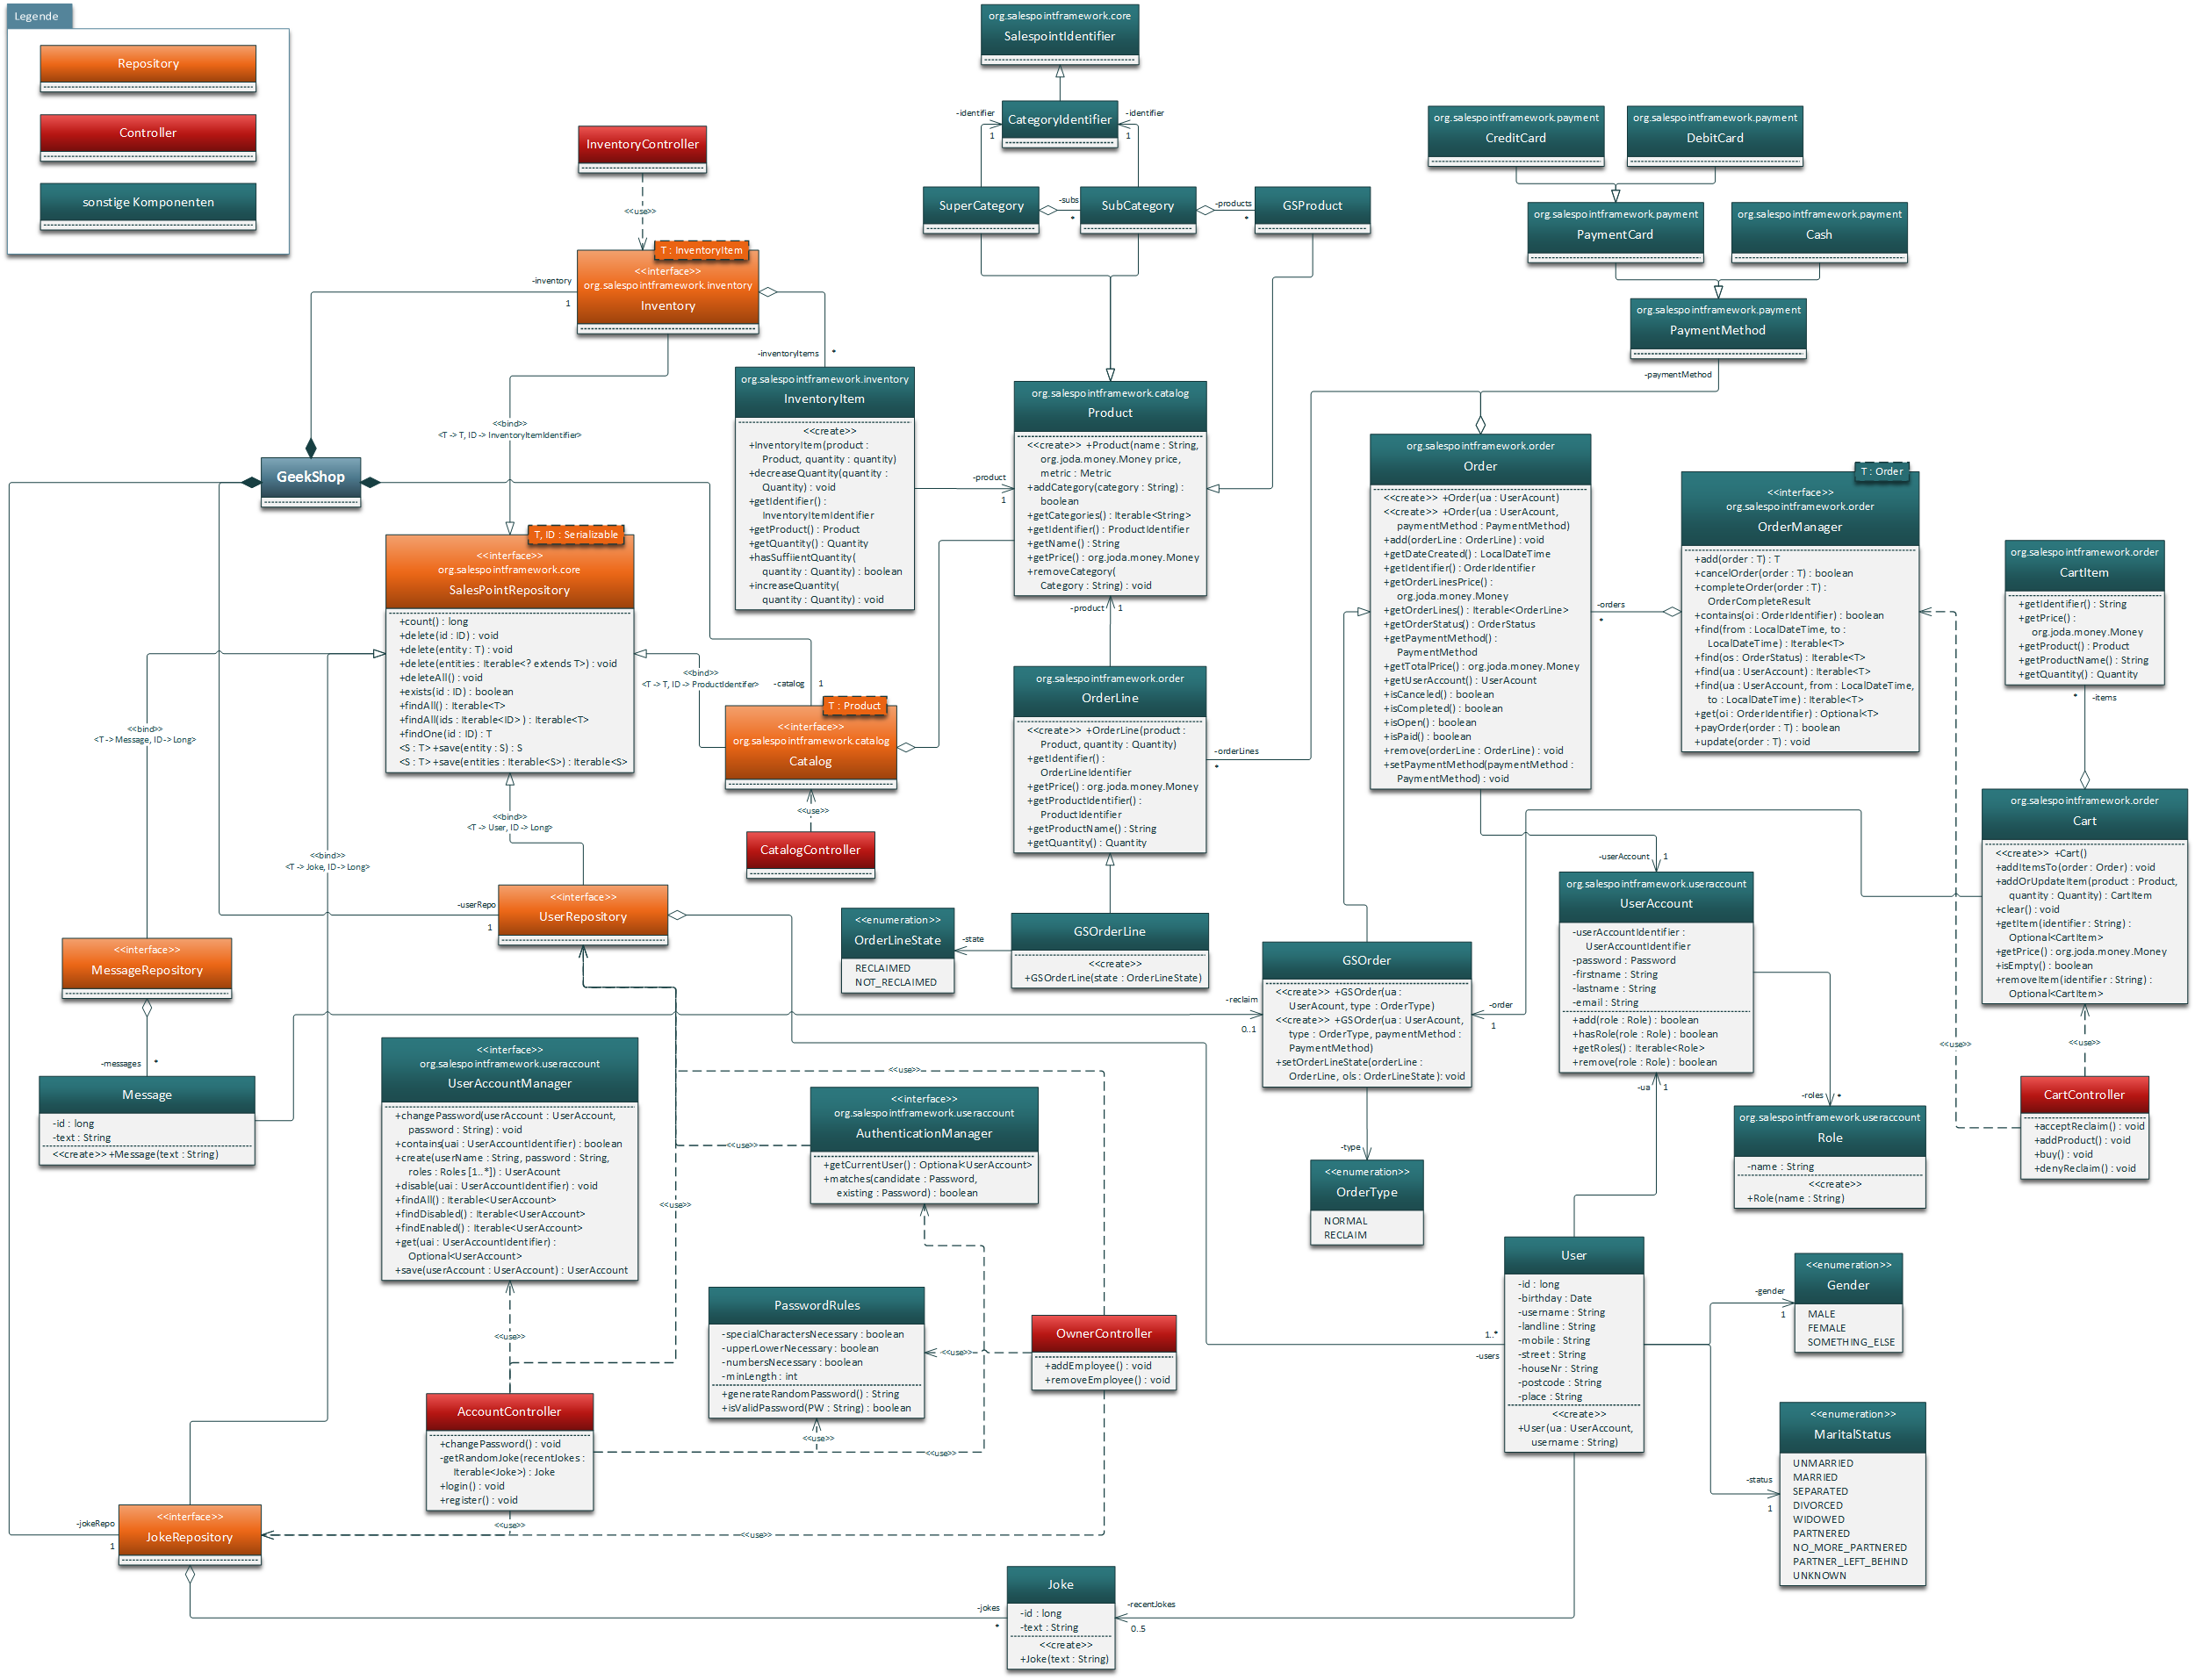
\includegraphics[scale=.131]{../../Entwurf/ekd_ood}}
\end{frame}

\subsection{Sequenzdiagramme}
\begin{frame}
\frametitle{Angestellten hinzuf\"ugen}
\center{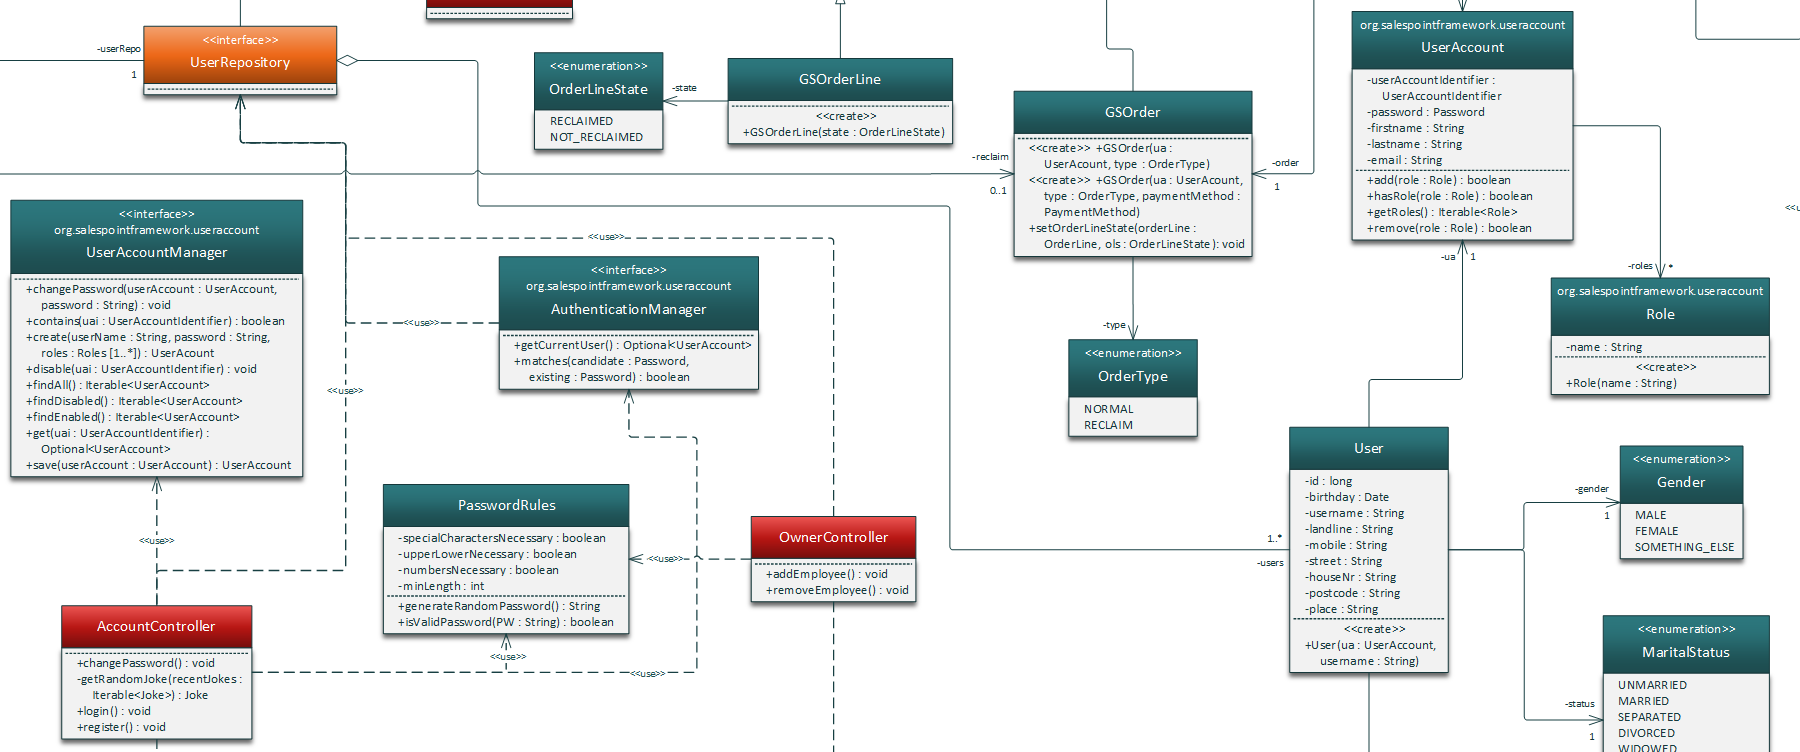
\includegraphics[width=\textwidth]{source/ekd_user}}
\end{frame}

\begin{frame}
\frametitle{Angestellten hinzuf\"ugen}
\center{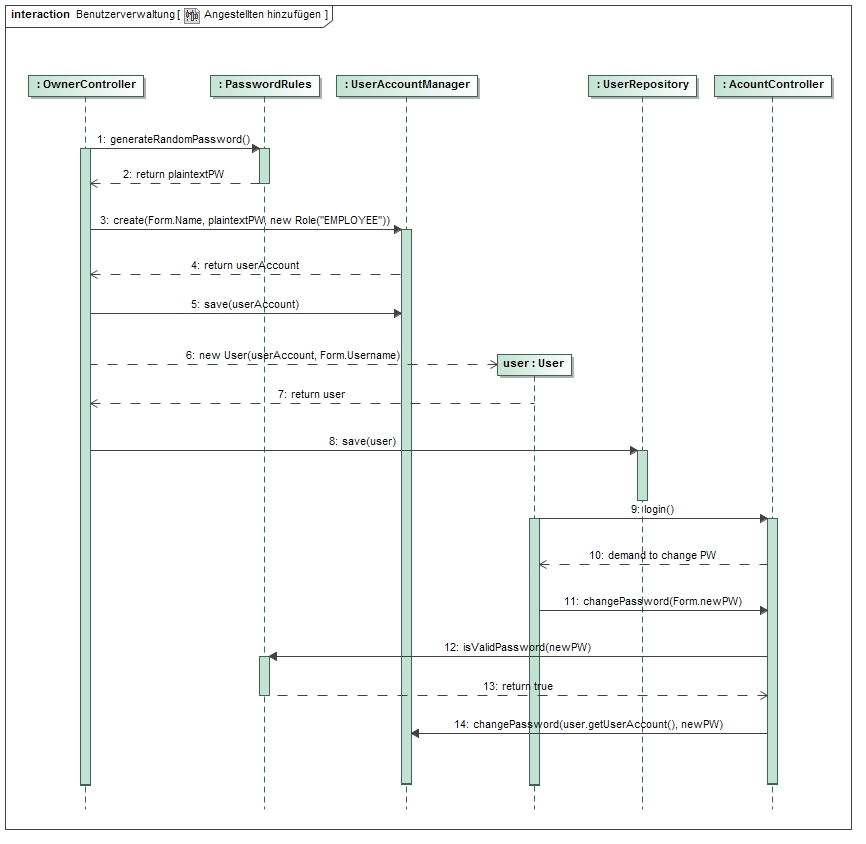
\includegraphics[scale=.23]{../../Entwurf/angestellten_hinzufuegen_ood}}
\end{frame}

\begin{frame}
\frametitle{Kaufvorgang}
\center{\includegraphics[width=\textwidth]{source/ekd_order}}
\end{frame}

\begin{frame}
\frametitle{Kaufvorgang}
\center{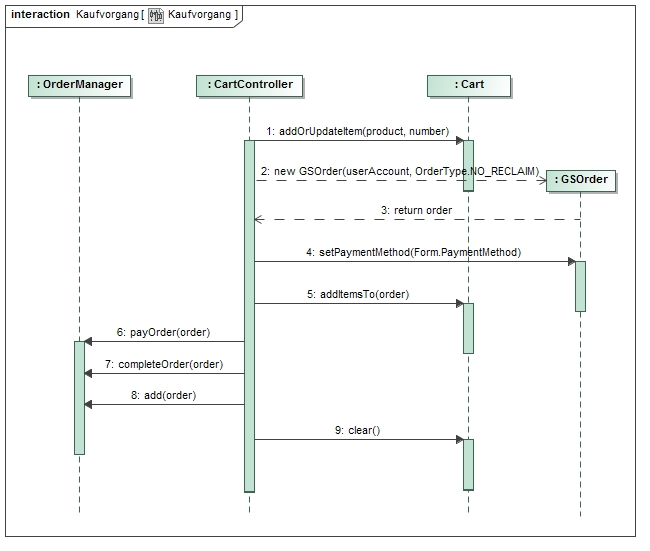
\includegraphics[scale=.35]{../../Entwurf/kaufvorgang_ood}}
\end{frame}

\begin{frame}
\frametitle{Reklamation}
\center{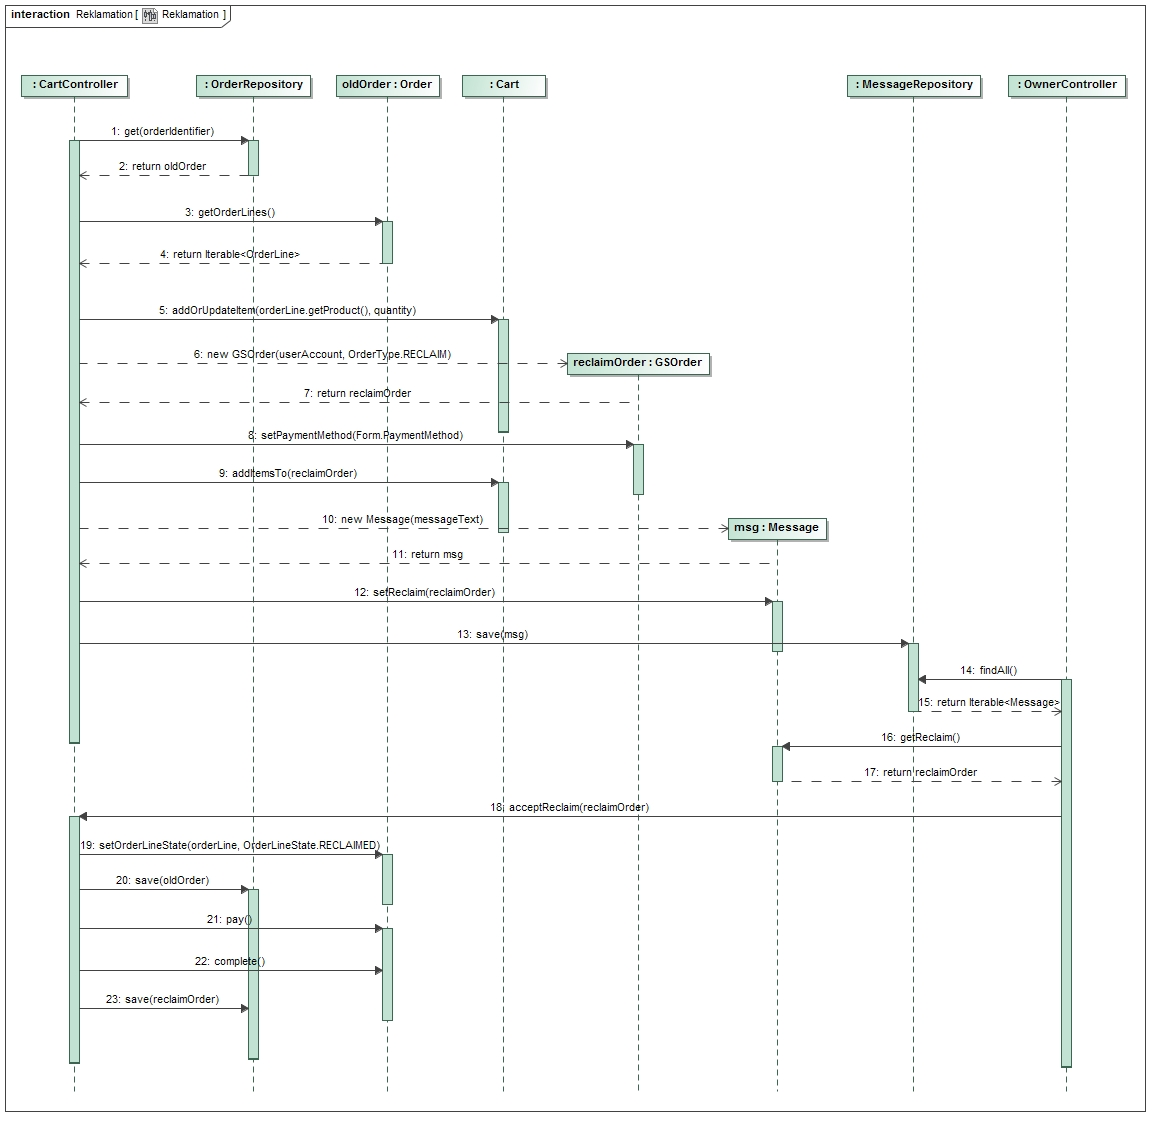
\includegraphics[scale=.16]{../../Entwurf/reklamation_ood}}
\end{frame}

\section{Dialoglandkarte}
\begin{frame}
\frametitle{Dialoglandkarte}
\center{\includegraphics[scale=.2]{../Pflichtenheft/images/dialoglandkarte}}
\end{frame}

\section{Prototyp}
\begin{frame}
\frametitle{Prototyp}
\center{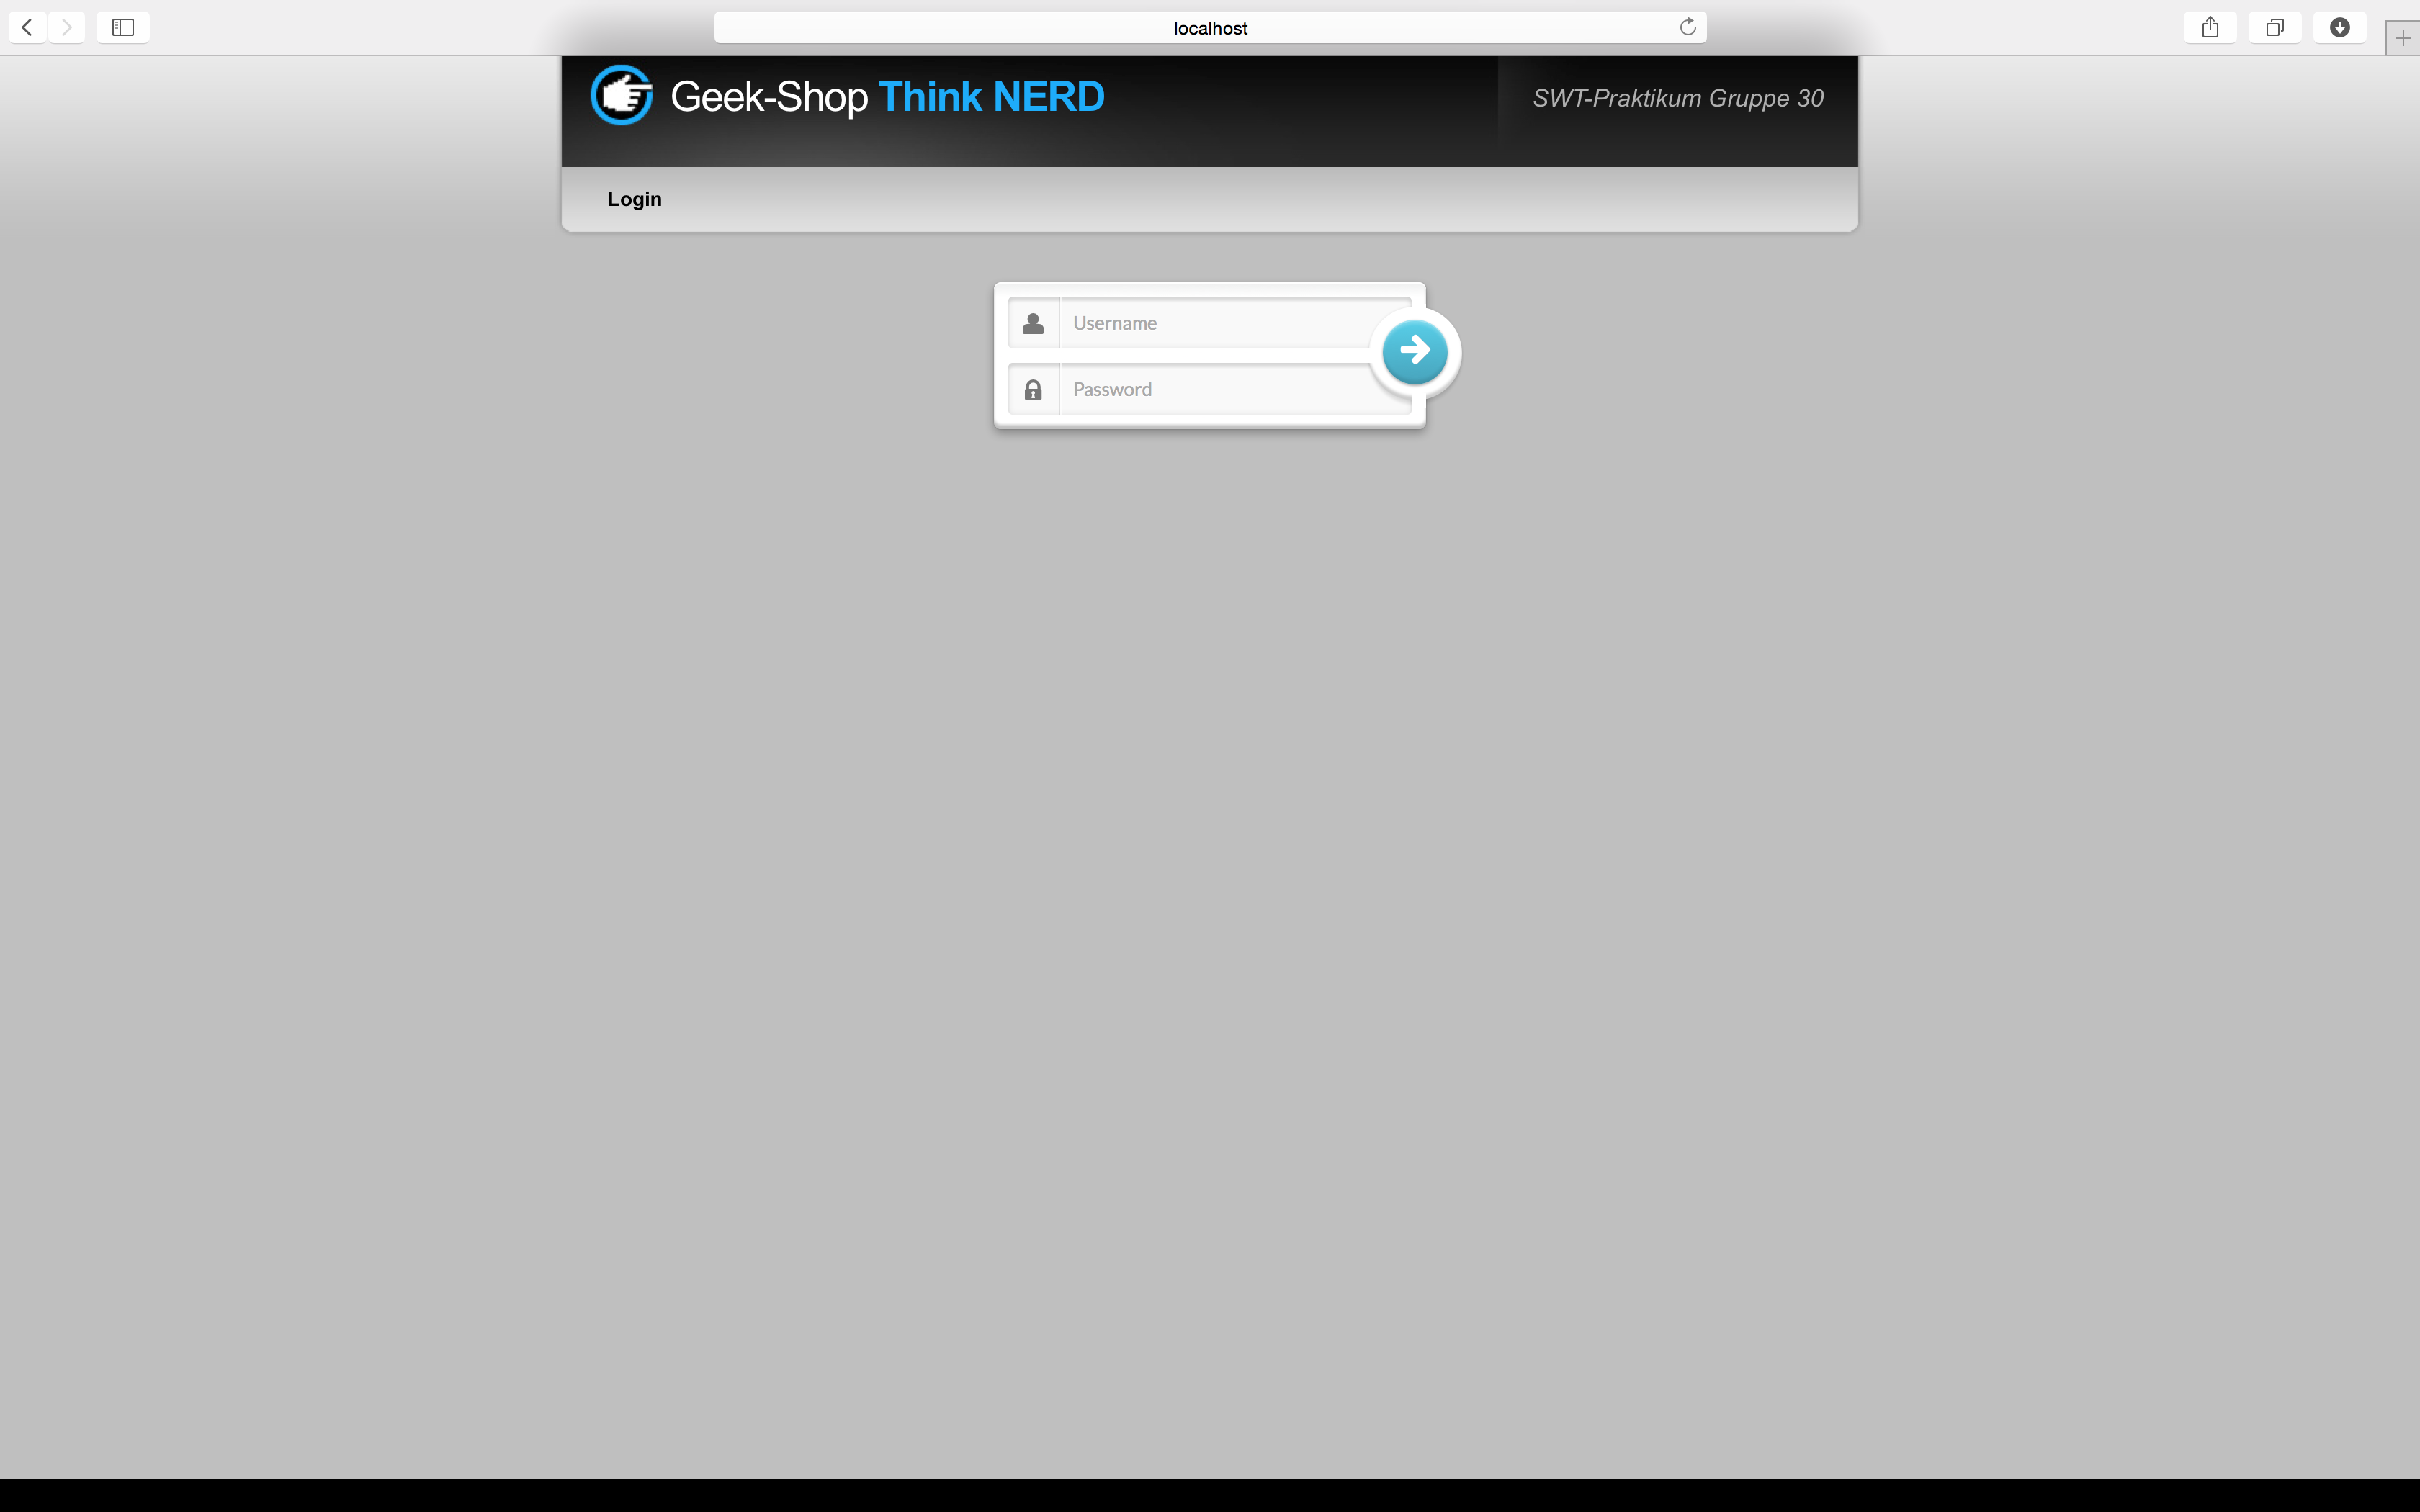
\includegraphics[scale=.175]{source/login}}
\end{frame}

\end{document}
